% !TeX spellcheck = en_US
\textbf{The Matrix-Vector Product}

Implement a function that takes as input a matrix $A \in \mathbb{R}^{m\times n}$ and a vector $x \in \mathbb{R}^{n}$ and then returns the matrix-vector product $Ax$.
\begin{enumerate}
	\item 
Implement the following four ways:
\begin{enumerate}	
	\item \textbf{Dense:} Input expected as \verb|numpy.ndarray|:\\
		  Assume that the matrix and the vector are delivered to your function as \verb|numpy.ndarray|.
	\begin{enumerate}
		\item Implement the matrix-vector product ``by hand'' using for loops, i.e., \textit{without} using numpy functions/methods.
		\item Implement the matrix-vector product using \texttt{A.dot(x)}, \verb|A@x|, \verb|numpy.matmul(A,x)| or \verb|numpy.dot(A,x)|. 
	\end{enumerate}
	\item \textbf{Sparse:} Matrix expected in \hyperref{https://en.wikipedia.org/wiki/Sparse_matrix#Compressed_sparse_row_(CSR,_CRS_or_Yale_format)}{}{}{CSR format}:\\
	Assume that the matrix is delivered to your function as \hyperref{https://docs.scipy.org/doc/scipy/reference/generated/scipy.sparse.csr_matrix.html}{}{}{\texttt{scipy.sparse.csr\_matrix}} object. The vector $x$ can either be expected as \verb|numpy.ndarray| or simply as a Python \texttt{list}. 	
	\begin{enumerate}
		\item Access the three CSR lists via \texttt{A.data, A.indptr, A.indices} and implement the matrix-vector product ``by hand'' using for loops.
		\item Implement the matrix-vector product using \texttt{A.dot(x)} or \texttt{A@x} . %Print the number of Gbytes which are needed to store the matrix in CSR format (have a look at: \texttt{A.data}, \texttt{A.indptr}, \texttt{A.indices}).
	\end{enumerate}
\end{enumerate}
\item \textbf{Test} your four different routines from above on the following matrix $A \in \mathbb{R}^{n \times n}$ with constant diagonals given by 
$$A = \begin{pmatrix}
2 & -1 		& 0  &\cdots & 0\\
-1 & 2 		& -1  &\ddots &  \vdots\\
0 & \ddots  		&\ddots   	 &\ddots  & 0 \\
\vdots    & \ddots  		&-1  	 &2 & -1\\
0 & \cdots 	&  0  &-1 & 2\\
\end{pmatrix} \in \mathbb{R}^{n \times n}$$
and the input vector $$x = (1,\cdots,1)^\top \in \mathbb{R}^n ~~~(\text{you can use:}~~ \verb|x = numpy.ones(n)|).$$ 
\begin{enumerate}
	\item Determine how $b:=A\cdot x \in \mathbb{R}^n$ looks like in this example in order to facilitate a test.
	\item Test whether your four routines compute the matrix--vector product correctly by checking $A\cdot x = b $.
	\item Use different values for the dimension $n$ (especially large $n\geq 10^5$ -- note that you may exceed your hardware capacities for the dense computations).
\end{enumerate}
\textit{Remark:} The matrix has ``$2$'' on the main diagonal and ``$-1$'' on the first off-diagonals.

\item For all cases:
\begin{enumerate}
	\item \textbf{Memory:} What is the number of Gbytes needed to store an $m \times n$ array of \texttt{floats}? Print the number of Gbytes which are needed to store the matrix in all cases.  \\
	\textit{Hint:} A number implemented as \texttt{float} in Python implements double precision and therefore needs \texttt{64} Bits of storage. For a \verb|numpy.ndarray| you can type \verb|A.nbytes| and for the \texttt{scipy.sparse.csr\_matrix} you can type \texttt{A.data.nbytes + A.indptr.nbytes + A.indices.nbytes}.
	\item \textbf{Computation times:} Measure the time which is needed in each case to compute the matrix-vector product for a random input vector \verb|x = numpy.random.rand(n)|. \\
	\textit{Hint:}  In the IPython shell you can simply use the \textit{magic function} \verb|%timeit| to measure the time for a certain operation. For example, you can type \verb|%timeit pythonfunction(x)|. Alternatively you can use the package \verb|timeit|.
\end{enumerate}
\end{enumerate}
%\begin{figure}[h!]
%	\centering
\begin{center}
		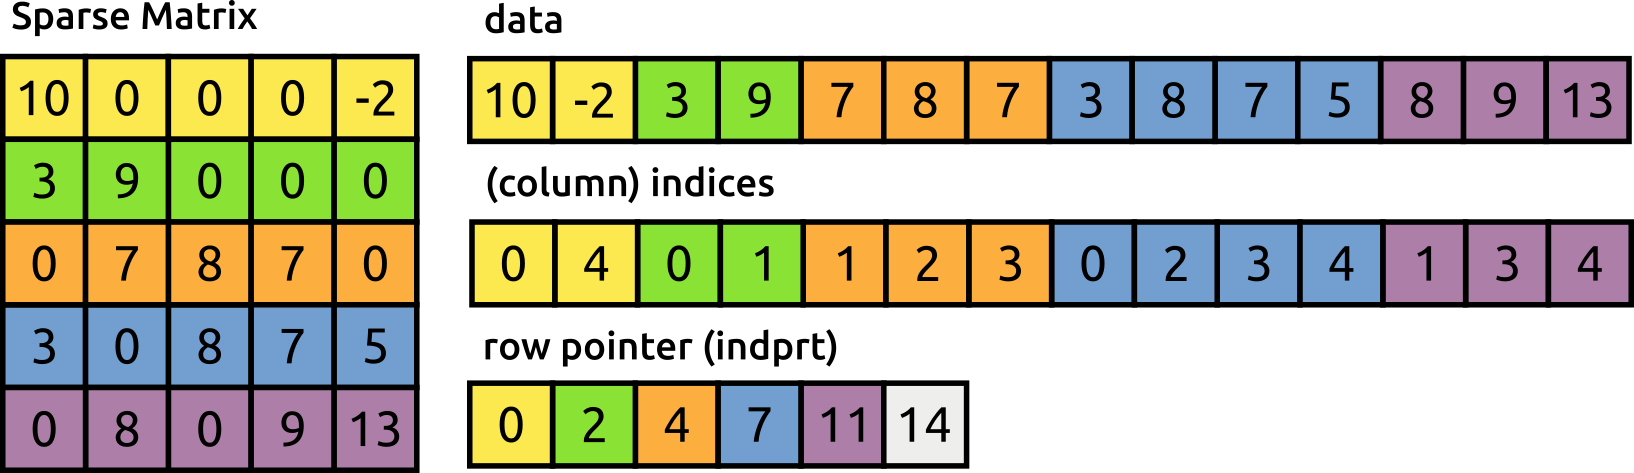
\includegraphics[width=0.8\linewidth]{csr-matrix}\\
		Example of a Matrix in CSR Format
\end{center}
%	\caption{Example of a Matrix in CSR Format}
%	\label{fig:csr-matrix}
%\end{figure}

%\begin{enumerate}
%	\item  Implement a function \verb|matfree(x)| which outputs the matrix-vector product $A \cdot x$ without using the matrix $A$ explicitly.
%\end{enumerate}